
\chapter{算法实现}

\section{概述}

摄像头拍摄的是彩色图像,如图\ref{fig:src}所示。从图上看出,不同电流表的数字形状和大小相同,给识别带来了方便。然而,数字只占整幅图像很小的一部分。电流表在黑色边框中,而电流表指针和电流表右侧也有黑色边框。防护玻璃表面有反光、灰尘,数字的黑色边框亮度不均匀,图像中又含有噪声。这些都给数字识别带来了干扰。因此,在识别数字前,必须首先减少噪声,排除无关部分的干扰。为此,本文将读数识别分成预处理、数字边框定位、数字分割和数字识别四个过程。其中预处理用于增强图像质量,数字边框定位通过找出黑色边框找出数字的大致位置,数字分割则精确地分割出数字的像素,数字识别则用于识别分割的数字。

\begin{figure}[h]
  \centering
  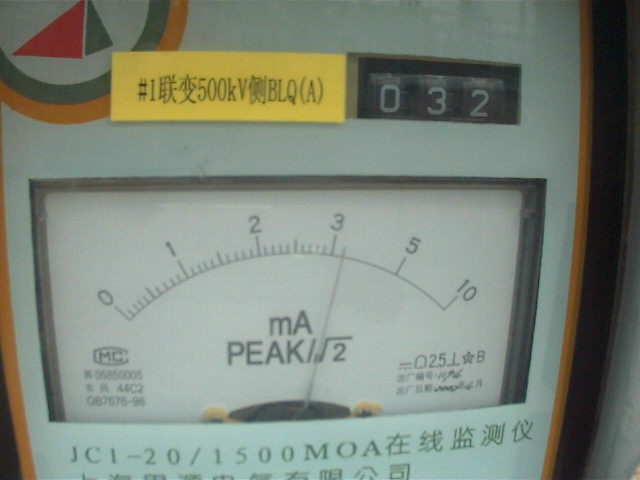
\includegraphics[scale=0.5]{src.png}
  \caption{原始图像}
  \label{fig:src}
\end{figure}

\section{图像预处理}

受光照条件和噪声等因素的影响,图像的质量不佳,不能直接用于数字识别\upcite{imgproc}。需要进行预处理,改善图像质量,从而更容易识别数字。本文采用的预处理方法先后有\emph{灰度化},\emph{高斯滤波}和\emph{直方图均衡}。

\subsection{灰度化}



由于待识别的数字在右上角,所以只需截取右上部分做后续处理,如图\ref{fig:rgb}所示。首先将彩色图像转换成灰度图像。这样做的原因是:
\begin{asparaenum}[(1)]
\item 灰度图像只有一个分量,比三分量的彩色图像更易处理;
\item 本文识别的数字边框为黑底白字,边框内绝大部分像素都是黑白颜色,灰度化后颜色基本没有变化。
\end{asparaenum}

本文使用OpenCV建议的加权平均法求出灰度图像,OpenCV给出的公式为$I=0.114R+0.587G+0.299B$。灰度图像如\ref{fig:gray}所示。

\begin{figure}[h]
  \centering
  \subfloat[彩色图像]{\label{fig:rgb}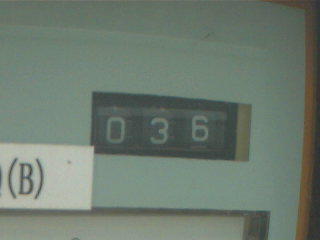
\includegraphics[scale=0.5]{rgb.png}}\hspace{1in}
  \subfloat[灰度图像]{\label{fig:gray}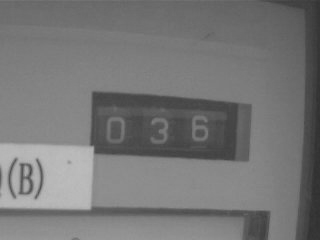
\includegraphics[scale=0.5]{gray.png}}
  \caption{灰度化}
\end{figure}

\subsection{高斯滤波}


灰度图像含有较多噪声,不利于提取目标,需要用图像平滑的方法减少噪声。观察发现,待处理图像的噪声以盐椒噪声为主,因此选用高斯滤波进行平滑滤波\upcite{imgproc}。在调用OpenCV的高斯滤波函数时,要指定高斯滤波模板的长宽,$\sigma$值和边界扩充类型。一般情况下,只需使用长宽相等的高斯滤波模板。模板尺寸越大,平滑的效果越好,但图像的边缘也越模糊。综合以上情况,将长和宽均设置为3。$\sigma$值的设定也有一定的要求。高斯函数在半径为$2\sigma$范围内的积分为0.95,故绝大部分权值集中在这个领域内。为了最大限度地发挥高斯滤波的效果,需要保证模板能覆盖这个邻域,故选择$\sigma=2/3$。边界扩充类型指将高斯滤波模板中心与图像边界重合,模板覆盖的部分像素超出图像边界时,这部分像素值的计算方式。一般的做法是将边界内的像素值复制到边界外。高斯滤波的效果如\ref{fig:gauss}所示。
\begin{figure}[h]
  \centering
  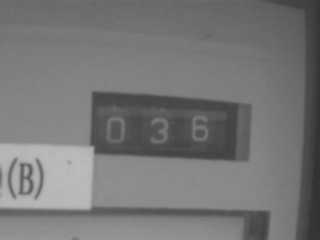
\includegraphics[scale=0.5]{gaussian.png}
  \caption{高斯滤波}
  \label{fig:gauss}
\end{figure}

\subsection{直方图均衡}


由于不同时间内光照条件不同,不同时间采集的图像的整体亮度不同。例如日光微弱时图像整体偏暗,日光强烈时图像整体偏亮。偏暗和偏亮的图像对比度不高,不利于识别。因此,采用直方图均衡化的方法增强图像的动态范围,从而达到增强图像整体对比度的效果。在进行直方图均衡化前,需要进行图像平滑。这是因为直方图均衡对图像的所有像素的灰度不加选择地加以扩充,因此噪声的灰度也被扩充,使原本灰度相近的区域灰度差距加大,对图像分割造成不利影响。因此本文把直方图均衡化放在高斯滤波后进行。

比较均衡化前的直方图\ref{fig:histsrc}和均衡化后的直方图\ref{fig:histequal}分别是均衡化前和均衡化后的直方图,可以发现均衡化后的直方图比均衡化前的直方图具有更宽的动态范围,每个灰度级上有大致相等的像素数。
\begin{figure}[h]
  \centering
  \subfloat[均衡化前的直方图]{\label{fig:histsrc}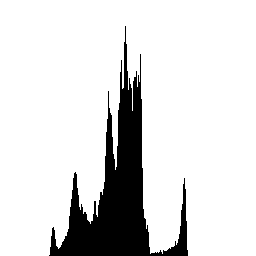
\includegraphics[scale=0.5]{histsrc.png}}
  \subfloat[均衡化后的直方图]{\label{fig:histequal}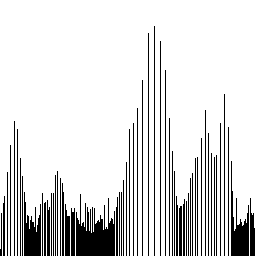
\includegraphics[scale=0.5]{histequal.png}}
  \caption{均衡化前后的直方图}
\end{figure}
直方图均衡化后的图像如图\ref{fig:equal}所示。经直方图均衡化后,不同时间的图像灰度分布大致相同,对于图像分割和识别是十分有益的。
\begin{figure}[h]
  \centering
  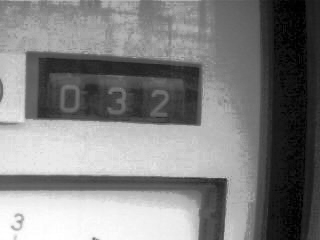
\includegraphics[scale=0.5]{equal.png}
  \caption{直方图均衡化}
  \label{fig:equal}
\end{figure}



\section{数字边框定位}

数字边框定位是电表读数识别的一个关键环节,也是较难的环节。数字边框内的数字是待识别的目标,数字边框外的图像则为无用信息。直接从原图中提取数字,难度大,准确率低。因此,应首先找出数字边框,去除无用的部分。观察图\ref{fig:equal}发现,数字边框周围有一些干扰区域,如右侧的电表边框和下侧的指针边框颜色灰度和数字边框的背景类似。这些干扰区域增加了分割的难度。

\subsection{二值化}

数字边框定位的第一步是二值化,即将原图分割为目标区域和背景区域,将目标区域的灰度设为255,背景区域的灰度设为0。观察图像发现,图像的各个区域内灰度差别较小,区域间灰度差别较大,适合用阈值法分割。阈值分割的关键是找到阈值。由于本文的灰度图像由大片的黑色和白色区域组成,可以使用Otsu算法分割阈值,

由式\eqref{eq:otsu}可得,Otsu算法需要对每个可能的灰度$t$计算$q_1(t),q_2(t),\mu_1(t),\mu_2(t)$四项。如果直接根据式\eqref{eq:musig}计算这四项,计算过程复杂而低效。为了简化计算,可以将式\eqref{eq:musig}改写成递推公式:
\begin{equation}
  \label{eq:recursive}
  \begin{aligned}
    q_t(t+1) &=q_1(t)+P(t+1)\\
    q_2(t+1) &=1-q_1(t) \\
    \mu_1(t+1) &=\frac{\mu_1(t)q_1(t)+(t+1)q_1(t+1)}{q_1(t+1)} \\
    \mu_2(t+1) &=\frac{\mu-q_1(t+1)\mu_1(t+1)}{q_2(t+1)}
  \end{aligned}
\end{equation}
递推公式\eqref{eq:recursive}含有总体均值$\mu$,需要在遍历$t$计算这四项之前计算。设定这四项的初值$q_1(0)=0,q_2(0)=1,\mu_1(t)=0,\mu_2(t)=\mu$,从$t=0$开始计算这四项,每增加一次$t$值,就更新这四项的值。如果小于某个$t$值的区间均值$q_1(t)$极小,则其方差$\mu_1(t)$极大,这个区间的像素极少,这样的$t$值必然不能作为分割点。同理,如果$t$值过大,导致大于$t$的区域的像素极少,同样不能作为阈值。因此计算$q_1(t)$和$q_2(t)$后,如果其中一项小于一个很小的门限,则这时的$t$值不能作为阈值,应直接进入下一轮循环。确保$t$值有效后,再用式\eqref{eq:sigb}更新组间方差$\sigma_B^2$,如果大于目前最大的$\sigma_B^2$值,则将阈值$t^{*}$更新为$t$。遍历$t$的所有取值后,即找出阈值$t^{*}$。分割结果是二值图像,如图\ref{fig:otsu}所示。从图上看出,数字也分割了出来,可以直接从图中找出数字。然而,这只是数字的初步分割。对于绝大多数电流表图像,这种初步分割得到的数字轮廓不准确,所以需要在数字边框定位后,在数字边框内的小块图像对数字进行精确定位。

\begin{figure}[h]
  \centering
  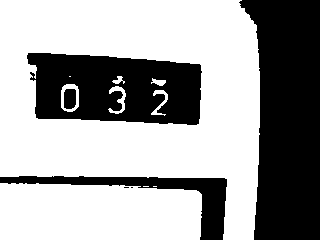
\includegraphics[scale=0.5]{otsu.png}
  \caption{Otsu算法}
  \label{fig:otsu}
\end{figure}


\subsection{连通成分筛选}

观察图\ref{fig:otsu}可得,二值化的图像黑色部分不仅包含数字边框,还包含其他几个区域,如电流表指针盘的边框和右侧的边框。这些区域需要去除,只保留数字边框。


由于这几个区域都是黑色区域,为了区分这几个区域,可以用连通成分标记算法给不同的区域赋予不同的标记。一般情况下,区域内可能有空洞或裂痕,连通成分标记可能失效。但这里的图像二值化的效果较好,区域内部不存在裂痕,适合用连通成分标记算法处理。本文选用\ref{sec:comp}节介绍的逐行扫描算法进行连通成分标记。逐行扫描算法使用并查集记录等价关系。扫描过程中算法对并查集进行大量的$\union$和$\find$操作,因此$\union$和$\find$操作的效率关系到算法的效率。

为优化$\find$和$\union$操作,可以使用如下两种策略。第一种策略是\emph{按秩合并}\upcite{alg},对任意元素$x$,它的\emph{秩}定义为从该结点到其后代结点的最长路径的边数的上界,记作$rank[x]$。当用$\make(x)$创建仅包含元素$x$的集合时,$rand[x]=0$。所有$\find(x)$操作不改变$rank[x]$。进行$\union(x,y)$操作时,比较结点$x$和结点$y$的祖先的秩,如果不相等,将秩较低的根结点指向秩较高的根结点,两者的秩不增加;如果相等,则任选一个根结点指向另一个根结点,并增加新的根结点的秩。另一种策略是\emph{路径压缩}\upcite{alg}。它用于$\find(x)$操作,将其访问的所有的结点都直接指向根结点。连通成分标记算法的结果如图\ref{fig:candidate}所示,不同区域已经用不同的灰度区分。

%用并查集使逐行扫描算法更加高效。算法第一次扫描,找到种子像素时,设定一个标号,并在并查集中创建一个只包含该标号的集合。在将标号传播到右下方的邻接点的过程中,如果发现两个不同的标号传播到同一个像素,只传播较小的标号,并将两个标号所在的集合合并。第一次扫描结束后,所有标号所在的集合均已确定。在第二次扫描时,将像素的标号改成该标号所在集合的代表标号。


\begin{figure}[h]
  \centering
  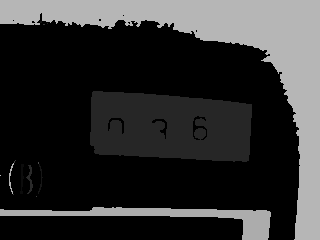
\includegraphics[scale=0.5]{candidate.png}
  \caption{连通成分}
  \label{fig:candidate}
\end{figure}


标记完各个连通成分后,下一步是从中找出数字边框。对这些连通成分进行分析。首先对连通成分进行初步分析,得到每个连通成分的基本特征,如像素数$n$和包围连通成分的最小矩形的长$L$和宽$W$等。在这些基本特征的基础上可以得到另一些特征。如长宽比$r=L/W$,面积$S=L\times R$等。再定义连通成分的区域密度为$\rho=n/S$。通过人工找出多幅图像内数字边框,综合它们的连通成分的基本特征的范围,得到数字边框对应的连通成分的各个特征具有如下范围:
\begin{equation}
  \label{eq:range}
  \begin{cases}
    8000  <  p  <  10000 \\
1.9  <  r  <  2.9 \\
0.6  <  \rho  < 0.9 
  \end{cases}
\end{equation}
因此,对每个连通成分计算这些特征值,发现落在式\eqref{eq:range}所示范围的,可以认定为数字边框。找出的数字边框如图\ref{eq:frame}所示。
\begin{figure}[h]
  \centering
  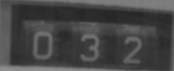
\includegraphics[scale=0.5]{frame.png}
  \caption{数字边框}
  \label{eq:frame}
\end{figure}

\subsection{倾斜校正}

因拍摄的角度问题,数字及其边框有一定的倾斜角度。因此找出数字边框后,为便于数字分割与识别,应对数字边框图像进行倾斜矫正。具体做法是先找出数字边框的上下两条横线,这两条横线的倾斜角度作为整个数字边框的倾斜角度,然后根据倾斜度旋转图像,使边框水平。

用边缘检测算子可以找出上下两条横线。由于数字边框较小,虚假的边缘对横线的倾斜角度有较大影响,边缘检测应尽量准确。为了提高边缘检测的准确度,减少虚假边缘,本文使用Canny边缘检测算子。OpenCV实现了边缘检测算子函数,但需要提供高低两个阈值和梯度的计算方式。由\ref{sec:edge}节可知,高低阈值用于Canny算子的非最大值抑制过程,只有高于这两个阈值的边缘才得以保留。这两个阈值可以在进行仪表自动识别前确定。具体做法是用Sobel算子或Prewitt算子求出原始图像的梯度图像,由于需要保留的边缘数字边框上下两条横线,因此找出横线上较高的幅值作为高阈值,较低的幅值作为低阈值。OpenCV提供了两种梯度计算方式,分别是按梯度定义给出的算式$|\nabla f|=\sqrt{f_x^2+f_y^2}$和梯度的近似计算$|\nabla f=|f_x|+|f_y|$。为了减少运算量,本文选择梯度的近似计算方法。边缘检测的结果如图\ref{fig:canny}所示。
\begin{figure}[h]
  \centering
  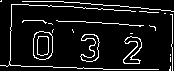
\includegraphics[scale=0.5]{canny.png}
  \caption{Canny算子}
  \label{fig:canny}
\end{figure}

边缘检测算子只能找到所有边缘点,还应从边缘点中找出上下两条横线。本文采用哈夫变换检测这些直线,将其倾斜度作为整个边框的倾斜度。在用OpenCV进行哈夫变换时,需要指定直线的参数$\theta$和$\rho$的量化间隔$\Delta\theta$和$\Delta\rho$。量化间隔太小,计算量过大,并将出现一条边缘线分裂成几条短线的情况;量化间隔太大,检测出的直线不准确。需要反复实验,找出最佳的量化间隔。用多组量化间隔进行哈夫变换,观察结果,最后找出最佳的量化间隔为$\Delta\theta=2^\circ,\Delta\rho=2$。然而,无论如何选取阈值,都无法避免边框断裂成几条直线。因此在计算直线倾斜角时,应该统计多条直线的倾斜角的平均值。求出倾斜度$\theta$后,再将边框图像绕中心按反方向旋转$\theta$角度,使整个边框处于水平位置。旋转后的图像如图\ref{fig:rotate}所示。
\begin{figure}[h]
  \centering
  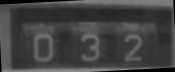
\includegraphics[scale=0.5]{rotate.png}
  \caption{旋转后的图像}
  \label{fig:rotate}
\end{figure}

\section{数字分割}


\subsection{二值化}


分割的第一步是二值化,将数字和背景的像素值设为255和0。观察图\ref{fig:rotate}发现,由于背景部分有反光,数字边框的背景灰度不均匀,不适合使用全局阈值法,应使用局部阈值法对平均灰度不同的小区域取不同的阈值。在局部阈值法的OpenCV实现中,OpenCV提供了两种计算阈值的方式,分别是用盒形滤波模板和高斯滤波模板计算加权平均值作为阈值\upcite{opencvref}。在OpenCV的实现中还可以指定参数$C$,表示将加权平均值加上$C$值作为阈值。因为反光处背景的灰度和数字相差不大,所以邻域内中心像素的权值应高于周围像素,选用高斯滤波模板计算加权平均值。经多次调整参数$C$发现,当$C=1.5$时,即将平均值加上1.5,可以获得较好的二值化图像。此时二值化图像的背景部分还有较多的噪声,数字部分内部有空隙,不利于分割和识别。由\ref{sec:morph}节可知,可以用形态学运算去除噪声并填补空洞。由于数字笔画较细,应先进行闭运算填补空隙,再用开运算减少噪声。为了保证形态学运算后数字的边界基本不变,本文选用的$3\times $十字形的形态学模板,如图\ref{fig:morph}所示。最后得到的二值化图像如图\ref{fig:framebin}所示,可以看出噪声并未完全消除。未消除的噪声需要在后续步骤中进行进一步处理。
\begin{figure}[h]
  \centering
  \includegraphics{cross.eps}
  \caption{形态学模板}
  \label{fig:morph}
\end{figure}

\begin{figure}[h]
  \centering
  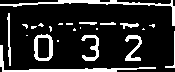
\includegraphics[scale=0.5]{framebin.png}
  \caption{数字边框的二值化图像}
  \label{fig:framebin}
\end{figure}

\subsection{数字定位}\label{sec:charseg}


求出二值化图像后,下一步是找出数字的位置。文献\cite{cookbook}推荐使用连通成分分析进行数字定位。然而,由于本文使用局部阈值法进行二值化,因而在二值化的图像中,数字可能断裂成互不连通的成分,因此不适合使用连通成分分析。综合以上情况,本文使用投影法定位数字。该方法能找出断裂的数字的各个部分。由于电表的数字在滚轮上,数字在竖直方向的位置不一定相同,因此先找出三个数字的在水平方向上各自的范围,然后在三个数字各自的水平范围内的图像做竖直投影。水平方向上的投影如图\ref{fig:projectx}所示。我们称这样的图为\emph{投影直方图}。
\begin{figure}[h]
  \centering
  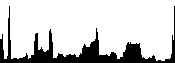
\includegraphics[scale=0.5]{projectx.png}
  \caption{水平方向投影}
  \label{fig:projectx}
\end{figure}

比较图\ref{fig:framebin}和\ref{fig:projectx}可得,二值图像的噪声点和线也投影到了横轴上。因此直接从含噪声的投影直方图中找出波峰容易出错。观察噪声对投影直方图的影响可以发现,噪声在投影直方图上形成各处均匀的背景噪声,使直方图整体抬高了。因此,投影直方图的噪声的关键,是找出背景噪声。减去这个幅度,就可以得到不含噪声的直方图。具体做法是,对投影直方图进行排序,找出位于中间处的像素数,作为背景噪声;然后将投影直方图各处均减去背景噪声,得到含噪声的直方图。这样做的理由是,因此在理想的投影直方图中,一半没有任何投影像素,另一半为数字形成的波峰。受背景噪声干扰,没有任何像素的地方都充满了背景噪声。因此,排序的投影直方图的前半部分,只有背景噪声没有数字投影。消除了背景噪声的投影直方图如图\ref{fig:proclear}所示。
\begin{figure}[h]
  \centering
  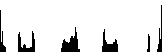
\includegraphics[scale=0.5]{proclear.png}
  \caption{消除背景噪声的投影}
  \label{fig:proclear}
\end{figure}

消除了噪声后,下一步是找出数字投影的波峰。观察直方图,可以发现数字的投影往往形成多个尖峰。例如数字“0”两侧的竖直线形成投影直方图的两个尖峰,中间部分形成一个较深的谷底。利用这个特点,我们可以使用类似于滞后阈值的方法找出波峰。具体做法是分别指定一个较高和较低的阈值,用高阈值找出数字投影的尖峰,然后在尖峰的两侧搜索高于低阈值的部分从而找出数字的完整的波峰。然后利用位置、宽度等信息去掉非数字形成的波峰。

用水平投影找出三个数字在水平方向的范围后,再用竖直投影找出三个数字在竖直方向的范围。由于竖直方向的投影只有一个数字,噪声对应的波峰没有数字的宽,因此,只需找出其中最宽的波峰,即可确定竖直方向的方位。经两次投影后,就可以分割出三个数字,如图\ref{fig:digit}所示。
\begin{figure}[h]
  \centering
  
\includegraphics{1.png}\hspace{1cm}
  
\includegraphics{2.png}\hspace{1cm}
  
\includegraphics{3.png}
  \caption{分割出的三个数字}
  \label{fig:digit}
\end{figure}

\section{数字识别}

由于不同电流表的数字形状和大小相同,没有旋转、扭曲、缩放等干扰,因此与前面的过程相比,数字识别是一个较为简单的过程。本文使用模板匹配法进行数字识别,因为模板匹配法具有不需要训练分类器,对数字断裂干扰不敏感等特点,适用于字符较少且字符形状和大小规范的情况。

\subsection{字符归一化}\label{sec:norm}

不同图片分割出的数字大小不一致,笔画粗细也各不相同,位置也有偏差,不利于识别。需要对数字做归一化处理,尽量减小相同数字的多幅图像的差异,进而在相同的标准下进行识别\upcite{vcpattern}。数字归一化的步骤有\emph{位置归一化}、\emph{尺寸归一化}和\emph{笔画粗细归一化}\upcite{vcpattern}。位置归一化的做法是,先计算数字的质心,然后以字符的质心为图像中心,平移图像。尺寸归一化的做法是将较待识别字符的长宽和模板做比较,求出在水平和竖直方向的缩放系数进行缩放运算。笔画粗细归一化相对复杂,因为既要求在尽量细化到笔画只有一个像素宽,又要保证不出现笔画断裂。这是两个矛盾的要求。鉴于待识别的数字形状简单,笔画很少,本文使用Hilditch细化算法\upcite{vcimg}。

Hilditch是简单直观的笔画细化算法,适用于处理二值字符图像,基本原理是逐层减少笔画宽度。为找出外层的笔画像素,Hilditch算法用如图\ref{fig:hilditchmask}所示的$3\times 3$模板判断某个像素是否为外层笔画像素\upcite{vcimg}。
\begin{figure}[h]
  \centering
  \includegraphics{hilditchmask.eps}
  \caption{Hilditch邻域}
  \label{fig:hilditchmask}
\end{figure}
将模板中心和字符像素重合,只有满足如下条件的像素,才判定为外层笔画像素,予以删除\upcite{vcimg}。
\begin{asparaenum}[(1)]

\item $x_1,x_3,x_5,x_7$不全为字符像素;
\item $x_1$到$x_8$不全为背景像素;
\item $x_1$到$x_8$中至少有两个是背景像素;
\end{asparaenum}

Hilditch算法对字符图像进行多轮扫描,每一轮标记待删除的像素,扫描结束后删除标记像素,直到某一轮未标记任何像素。本文的字符图像像素很少,笔画简单,多次扫描的运算量也不大。

\subsection{模板匹配}

不同电流表上的字符大小和形状相同,没有旋转和变形等干扰。数字的黑色背景光照不均匀,导致分割时数字易出现断裂。在这种情况下,适合使用模板匹配法进行数字识别。使用模板匹配法需要制作模板。具体做法是从\ref{sec:charseg}节得到的数字中,找出大小、形状和偏离方向最理想的,按\ref{sec:norm}节的方法统一成$16\times 27$的模板(大部分数字尺寸都在$16\times 27$左右),作为模板。其中,数字“1”不宜使用模板匹配,因为数字“1”比其他数字窄,如果进行归一化,数字“1”的横向拉伸形变非常严重。因此,在模板匹配前,先找出较窄的数字字符图像,通过检测是否为竖直直线确定是否为“1”。

模板匹配的关键是找出待识别数字和模板的差距。这个差距可以用Hausdorff距离度量\upcite{vcimg2}。设$A$是待识别图像的数字部分像素集合,$B$是模板的数字像素的坐标集合,则Hausdorff距离$H(A,B)$定义如下:
\begin{equation}
  \begin{aligned}
    h(A,B)&=\max_{a\in A}\min_{b\in B}||a-b||\\
    h(B,A)&=\max_{b\in B}\min_{a\in A}||a-b||\\
    H(A,B)&=\max(h(A,B),h(B,A))
  \end{aligned}
  \label{eq:hausdorff}
\end{equation}

由式\eqref{eq:hausdorff}可得,计算Hausdorff距离的具体做法是,先找出待识别数字和模板的数字部分的所有像素坐标,然后对于待识别数字的所有坐标,在模板中找出距离最近的坐标,然后取其中最大距离作为两者的Hausdorff距离。取Hausdorff距离最小的模板数字为识别的结果。

\section{实验结果}

为验证本文提出方法的效果,对不同角度不同光照条件下的电流表图像进行了试验。图\ref{fig:meter2}是另一幅电流表图像,图\ref{fig:frame2}是倾斜校正后的数字边框图像,图\ref{fig:digits2}是分割出的三个数字的图像,图\ref{fig:model2}是三个数字的图像分别匹配的三个模板,最终识别结果为036。

\begin{figure}[h]
\centering
  \subfloat[原始图像]{\label{fig:meter2}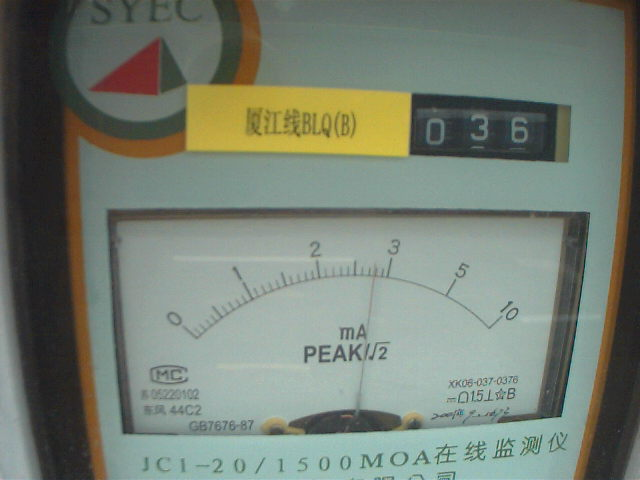
\includegraphics[scale=0.5]{14.png}}\\
\subfloat[数字边框]{\label{fig:frame2}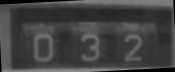
\includegraphics[scale=0.5]{frame2.png}}
\hspace{2cm}
\subfloat[分割的数字]{
  \label{fig:digits2}
  
\includegraphics{digit1.png}\hspace{0.5cm}
  
\includegraphics{digit2.png}\hspace{0.5cm}
  
\includegraphics{digit3.png}}\hspace{2cm}
\subfloat[三个数字模板]{
  \label{fig:model2}
  
\includegraphics{model0.png}\hspace{0.5cm}
  
\includegraphics{model3.png}\hspace{0.5cm}
  
\includegraphics{model6.png}}
\caption{另一张电流表图像的识别过程}
\end{figure}
本文对对47张不同角度不同光照条件下的电流表图像,共141个数字进行了试验。本方法正确识别了其中40张图片共120个数字,识别率为85.1\%。在未正确识别的7张图像中,其中4张是因为数字边框定位不准确,另外2张是因为数字边框图像二值化的效果不理想,最后1张是因为将竖直干扰线误认为数字“1”。影响电流表读数识别率的主要因素有
\begin{inparaenum}[(1)]
\item 电流表的防护玻璃和数字边框的反光较严重;
\item 电流表的防护玻璃灰尘较多;
\item 极少数摄像头未对焦。
\end{inparaenum}
因此,需要在该方法的基础上进行改进,找出更好地减少干扰和噪声的方法,提高识别率。

\section{本章小结}

本章的主要工作是对单个的数字字符图像进行识别。识别的第一步是进行归一化处理,包括位置归一花、尺寸归一化和笔画粗细归一化。然后用数字模板,利用Hausdorff距离衡量待识别像素和模板的差距,选择差距最小的模板对应的数字作为识别结果。该方法简单直观,对本文的电流表图像有较好的识别效果,但仍需要改进,以识别噪声干扰较严重的图像。
%%% Local Variables: 
%%% mode: latex
%%% TeX-master: "thesis"
%%% End: 
